\documentclass[12pt]{article}
% ---------------------------------
\usepackage{sbc-template}
\usepackage{float}
\usepackage{subcaption}
\usepackage{color, graphicx, url, xurl}
% ---------------------------------
% \usepackage{caption}
% \usepackage{subfigure}
\usepackage{multicol}
% ---------------------------------
\usepackage{longtable}
\usepackage[table,xcdraw]{xcolor}
\usepackage{amsmath, amssymb}
\usepackage{indentfirst}
\newcommand{\quotes}[1]{``#1''}
% ---------------------------------
\usepackage{hyperref}
% ---------------------------------
%Preambulo
\usepackage{array}
\usepackage{multirow}
\usepackage{booktabs}
\usepackage{lscape}
\usepackage{rotating}
\usepackage{tabulary}

\usepackage[brazil]{babel}   
\usepackage[utf8]{inputenc}
%\usepackage[latin1]{inputenc} 
% ---------------------------------
\graphicspath{{./img/}}
% ---------------------------------
\sloppy
\title{Comparação de Métodos baseados em Redes Convolucionais para Classificação de Fava}
\author{Erico Andre da Silva\inst{1}}
\address{Departamento de Estatística e Informática -- Universidade Federal Rural de Pernambuco\\ Rua Dom Manuel de Medeiros, s/n, - CEP: 52171-900  -- Recife -- PE -- Brasil
\email{erico.andre@ufrpe.br}}
\begin{document} 
\maketitle
% ---------------------------------
\begin{resumo} 
A cultura da fava tem recebido pouca atenção por parte dos órgãos de pesquisa e extensão, o que tem resultado em limitações do conhecimento das características agronômicas da cultura. Isso tem afetado a precisão em classificá-las. Tal classificação é de grande importância porque a identificação correta de plantas permite boa resposta da cultura em termos de produtividade e comportamento em diferentes condições ambientais. Neste contexto de informações limitadas sobre as características apresentamos uma solução que aplica o poder da visão computacional à agronomia, que visa melhorar a produtividade, reduzir desperdícios e auxiliar na tomada de decisões e na seleção de cultura que mais se adequá a uma região em particular. As técnicas de visão computacional são um conjunto de métodos utilizados para interpretar imagens, extraindo padrões e características. Visando contribuir com esse cenário de desenvolvimento tecnológico do setor do agronômico, este trabalho compara algumas das abordagens de classificação supervisionada para identificação de forma automática de espécies de favas. O escopo deste trabalho consiste em classificar imagens de mudas geradas por produtores rurais em duas categorias de favas: orelha de vó e cearense. A partir das comparações realizadas entre métodos de classificadores que utilizam redes convolucionais como extratores de características com diferentes classsificadores como máquina de vetores de suporte (SVM), arvore de descição e mlp, para ao final apresentarmos a melhor métodologia para automatizar a classificação das imagens de favas.
\end{resumo}
\section{Introdução} 

%A agricultura faz parte do setor primário da economia sendo fornecedor de alimento e de matéria-prima. Com a modernização e profissionalização, o setor deu um salto de importância na economia Brasileira. Atualmente é responsável por quase um quarto do Produto Interno Bruto (PIB)~\cite{FieldView}, e praticamente metade das exportações do país. 

A fava (\textit{Phaseolus lunatus} L.) também conhecida como feijão-lima ou feijão-fava é uma leguminosa cultivada em quase todas as regiões do mundo, sendo que no Brasil possui ampla distribuição em todo o território, principalmente no Nordeste, é uma das quatro espécies do gênero \textit{Phaseolus} exploradas comercialmente. A espécie foi domesticada na América do Sul ou Central, ou em ambas, e é subtropical \cite{zimmermann1988origem}. É uma das principais leguminosas cultivadas na região tropical e apresenta potencial para fornecer proteína vegetal à população, diminuindo a dependência quase exclusiva dos feijões do grupo carioca \cite{vieira1992cultura}. 

%A cultura da fava apresenta-se como fonte de renda e alimento, sendo um recurso natural disponível e resistente aos períodos de seca \cite{revistacultivar:2015}. Permitindo que comunidades rurais, desestimuladas pela exploração agropecuária limitada principalmente pela falta de água, possam recuperar o desejo de permanência no campo, possibilitando melhoria na qualidade de vida, segurança alimentar e nutricional para a agricultura familiar apesar das adversidades climáticas.

%Destacada a importância do feijão-fava à agricultura familiar, buscamos classificar de forma precocemente as mudas, evitando assim o desperdício de tempo e recurso com variedades que tenham uma baixa produtividade. Pois foi verificado que as mudas de feijão-fava são praticamente idênticas nas etapas iniciais tornando difícil mesmo para especialistas classificá-las.

A humanidade vem busca por meios que maximize o processo agrícola, evitando disperdi-cios e aumentando a produtividade agrícola, com a classificação das mudas de forma rápida e correta e possível escolher o melhor manuseio e um maior controle da produção.

A importância de se identificar as espécies de fava se dá porque cada variedade tem características que se diferem uma das outras como o tamanho de vagens e quantidade de grãos que podem variar para mais ou menos por safra, já a variedade orelha de vó tem o maior comprimento de suas vagens e maior peso de sementes que variedade fava-cearense. A escolha dessas duas espécies foi para resolver um problema do curso de agronomia da Universidade Federal Rural de Pernambuco (UFRPE). Que era classificar de forma rápida e precisa as variedades de Fava Orelha de Vó e Fava Cearense. 

Espera-se por meio desta pesquisa elaborar um métodos baseados em redes convolucionais com extrator de características na classificação de variedades de fava. Este trabalho foca-se na construção de um agente classificador utilizando redes convolucionais como extrator de características em diferentes abordagem de classificadores para distinguir espécies de feijão-lima ou feijão-fava, dentre elas a fava cearense e a orelha de vó auxiliando o agricultor na escolha do manejo adequado a espécie classificada.

%Espera-se por meio desta pesquisa contribuir com o processo de classificação de determinadas variedades de fava como orelha de vó e fava Cearense, através da imagens podem ser obtidas a partir de dispositivos portáteis, trazendo economia com essa automação, neste contexto, a análise de imagens tem função valiosa ao transformar os dados coletados no campo em informações úteis na tomada de decisão dos agricultores com a construção de um classificador automático.

 \label{sec:introducao}
\section{Comparação de Métodos baseados em Redes Convolucionais para Classificação de Fava}

\subsection{Aquisição das imagens e pré-processamento}

As imagens foram disponibilizadas por um aluno do curso de agronomia da Universidade Federal Rural de Pernambuco, que apresentou o seguinte questionamento se era possível classificar as mudas de feijão-fava já que elas eram quase idênticas utilizando métodos de aprendizado computacional. O conjunto possuí duas categorias de feijão-fava as Fava Cearense e Fava Orelha de Vó, totalizando 229 imagens, sendo 109 de Fava Cearense figura~\ref{fig:fava_cearens}, e 120 de Fava Orelha de Vó figura~\ref{fig:fava_Orelha_vo}.

\begin{figure}[H]
\centering
\begin{subfigure}[b]{0.3\textwidth}
\centering
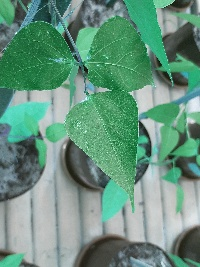
\includegraphics[width=\textwidth]{20191018_085120.jpg}
\caption{Cearense}
\label{fig:fava_cearens}
\end{subfigure}
\begin{subfigure}[b]{0.3\textwidth}
\centering
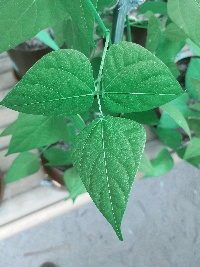
\includegraphics[width=\textwidth]{20191018_082656.jpg}
\caption{Orelha de Vó}
\label{fig:fava_Orelha_vo}
\end{subfigure}
\end{figure}

Devido a quantidade limitada de imagens utilizados nesse trabalho, as operações de acréscimo de dados (data augmentation), para aumentar a quantidade e a diversidade dos dados do conjunto de imagens, para evitar o overfitting da rede e garantir a sua generalização. Os métodos descritos foram implementados em Python, utilizando as bibliotecas Opencv (Open Source Computer Vision Library)~\footnote{ \url{https://opencv.org/about/}}, uma biblioteca de software de visão computacional e aprendizado de máquina de código aberto disponível em Python. As manipulação nas imagens foram: espelhamento horizontal e vertical, variação do nível de brilho, foi aplicado cinco transformações mais a copia da imagem original dando um total de seis gerada a partir de uma única imagem. Após esta etapa, o novo conjunto de imagens que foi gerada ficou com 654 imagem de Fava Cearense e 720 imagens de Orelha de Vó, totalizando 1374 imagens~\footnote{  \url{https://github.com/ericoandre/reconhecimento_padroes}}. A tabela~\ref{tabela:dataset1} mostra total das imagens antes e depois do o acréscimo de dados (data augmentation).

\begin{figure}[H]
\centering
\begin{subfigure}[b]{0.3\textwidth}
\centering
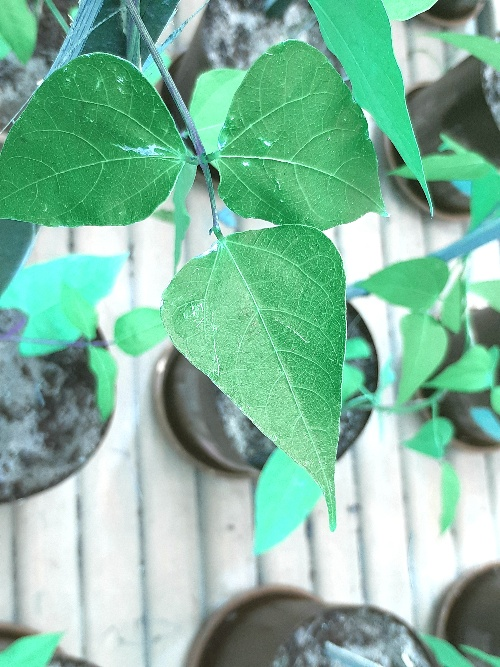
\includegraphics[width=\textwidth]{fava_cearense_augmented1.jpg}
\caption{Imagem com variação no brilho}
\label{fig:fava_cearense_augmented-1}
\end{subfigure}
\begin{subfigure}[b]{0.3\textwidth}
\centering
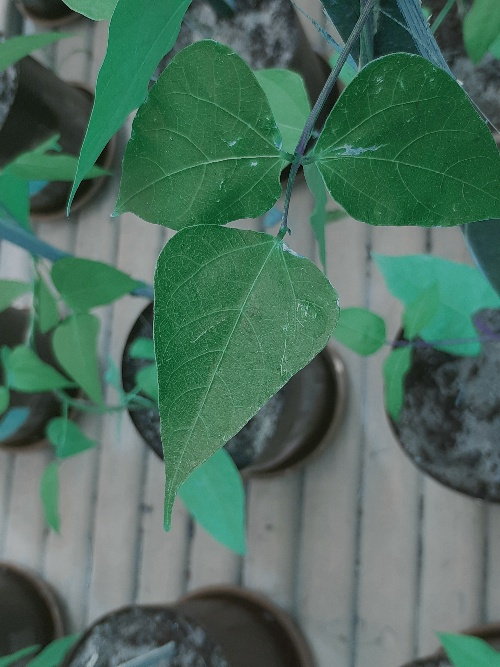
\includegraphics[width=\textwidth]{fava_cearense_augmented2.jpg}
\caption{Variação no brilho e flip horizontal}
\label{fig:fava_cearense_augmented-2}
\end{subfigure}

\begin{subfigure}[b]{0.3\textwidth}
\centering
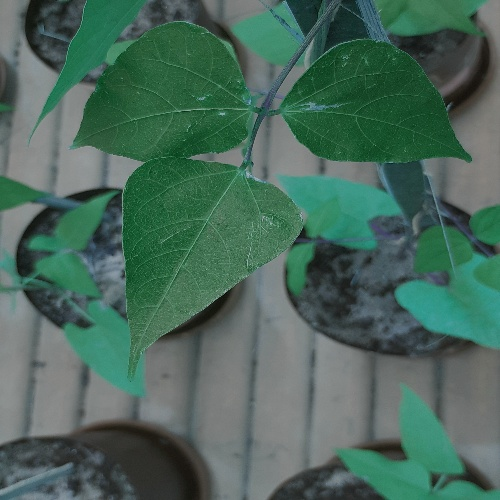
\includegraphics[width=\textwidth]{normal.jpg}
\caption{Imagem com variação no brilho}
\label{fig:geometrica_fava_cearense_augmented-1}
\end{subfigure}
\begin{subfigure}[b]{0.3\textwidth}
\centering
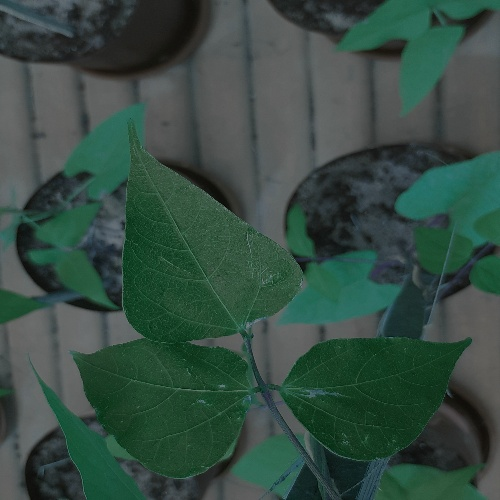
\includegraphics[width=\textwidth]{virada.jpg}
\caption{Variação no brilho e flip vertical}
\label{fig:geometrica_fava_cearense_augmented-2}
\end{subfigure}
\end{figure}

Técnica que ajuda na melhoria do modelo que é o acréscimo de dados (data augmentation) citada anteriormente. Todas as imagens possuem 3456 pixels de largura x 4608 pixels de altura, o que totaliza 47.775.744 atributos, que são provenientes dos três canais. Devido às limitações de hardware disponíveis, para que o treinamento dos algoritmos, foi necessário reduzir o tamanho da imagens em 200 pixels de largura x 267 pixels de altura, este é o menor valor obtido que não afeta a qualidade das imagens, o que resultou em 160.200 atributos para cada imagem, a figura~\ref{fig:geometrica_fava_cearense_augmented-1} e figura~\ref{fig:geometrica_fava_cearense_augmented-2} são imagens geradas com o método de acréscimo de dados onde seu tamanho foi reduzidos.

\begin{table}[H]
\centering
\begin{tabular}{ |c|c|c|c| } 
\hline
\textbf{Conjunto} & \textbf{Fava Cearense} & \textbf{Orelha de Vó} & \textbf{Total}  \\ [0.5ex]
\hline Imagens Originais & 109 & 120 & 229 \\
\hline Imagens Aumentadas & 654 & 720 & 1374 \\ \hline
\end{tabular}
\caption{Distribuição dos conjuntos de imagens}
\label{tabela:dataset1}
\end{table}

\subsection{Rede Neural Convolucional}

Uma Rede Neural Convolucional (CNN do inglês Convolutional Neural network ou ConvNet) é uma variação das rede neural feedforward de Múltiplas Camadas~\cite{BISHOP}, foi inspirada no processo biológico de visão dos seres vivos. Capaz de aplicar filtros aos dados, mantendo a relação de vizinhança entre os pixels da imagem ao longo do processamento da rede (VARGAS; PAES; VASCONCELOS, 2016). 

A arquitetura inicia proposta neste estudo consiste em quatro tipos básicos de camadas: 2 camada de convolução (Convolutional Layer) com filtros de tamanho 3×3 e 2x2, 1 camada de subamostragem (Subsampling Layers ou Pooling Layers), 1 camada de Dropout e por fim a totalmente conectadas (Fully Connected Layers), como mostrada na figura~\ref{fig:arquitetura_cnn_}, a tabela~\ref{tabela:hiperparametros_cnn} mostra as distribuições dos hiperparâmetros que foram utilizado selecionados pela busca aleatória  ~\cite{Bergstra_James}.

\begin{figure}[H]
\centering
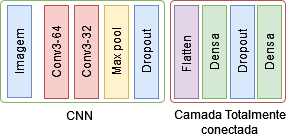
\includegraphics[width=0.5\textwidth]{CNN.png}
\caption{Arquitetura da CNN}
\label{fig:arquitetura_cnn_}
\par\medskip\selectfont\textbf{Fonte:} Elaborada pelo autor (2022) \par\medskip
\end{figure}

\begin{table}[H]
\centering
\caption{Hiperparâmetros do Modelo Inicial}
\label{tabela:hiperparametros_cnn}
\def\arraystretch{1.2}
\begin{tabular}{@{}lrrr@{}}
\toprule
{\textbf{Algoritimos}} & {\textbf{Hiperparâmetros}} & {\textbf{Distribuição de Probabilidade}}  \\
\midrule
CNN MLP & dropout & uniforme em \{0.5, 0.6, 0.7, 0.8, 0.9, 0.10, 0.11, 0.12\} \\ 
CNN MLP & neurônios & uniforme em \{32, 64, 128, 256\} \\ 
CNN MLP & ativação & uniforme em \{relu, sigmoid\} \\ 
CNN MLP & épocas &  uniforme em [50; 500] \\ 
CNN MLP & tamanho do batch &  uniforme em \{16, 32, 64, 128\} \\ 
CNN MLP & otimizador &  uniforme em \{adam, sgd, rmsprop, nadam\} \\ 
\bottomrule
\end{tabular}
\end{table}

Foi separada uma sub amostra de 30\% do conjunto de 1374 imagens totalizando 413 imagens, que foram utilizadas na validação dos modelos. Após isso, avaliação da rede convolucional, através da matriz de confusão notamos que das 413 acertou 182 da classe fava Cearense e 212 de fava Orelha de vó e teve instâncias teve 19 erros obtendo uma precisão de 0.94, com uma cobertura de 0.96 e a Área sob a curva AUC de 0.966.

Na tabela~\ref{tabela:hiperparametros_best_models_}, mostra os hiperparâmetros relacionado a melhor CNN, obtidos através da seleção de modelos.

\begin{table}[H]
\centering
\caption{Hiperparâmetros do Melhor Modelo de CNN }
\label{tabela:hiperparametros_best_models_}
\def\arraystretch{1.2}
\begin{tabular}{@{}lrrr@{}}
\toprule
{\textbf{Algoritimos}} & {\textbf{Hiperparâmetros}} & {\textbf{Variação}}  \\
\midrule
CNN MLP & epépocasochs & 364 \\ 
CNN MLP & tamanho do batch & 16\\ 
CNN MLP & otimizador & adam \\
CNN MLP & ativação & relu \\
CNN MLP & neurônios & 128 \\
CNN MLP & dropout & 0.1 \\
\bottomrule
\end{tabular}
\end{table}


\subsection{CNN como Extrator de Características}

% para ajudar o agricultor na difícil etapa de classificar nos estágios iniciais as diferentes espécies de feijão-fava, cada espécies tem diferentes comprimento das sementes tempo de colheita, manejo. Assim foi abordadas três comparações utilizando CNN, descritas individualmente na sequência:

% \begin{figure}[H]
% \centering
% 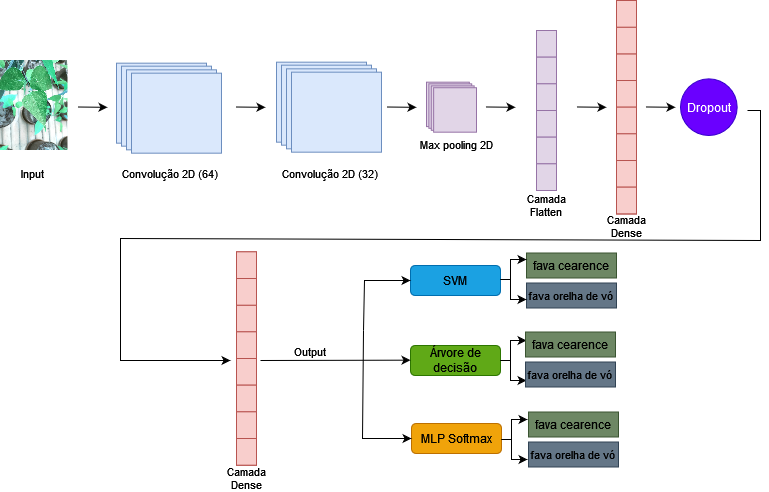
\includegraphics[width=.8\textwidth]{Arquitetura-CNN.png}
% \caption{Arquitetura proposta para a detecção automatizada de mudas \textit{feijão-fava}}
% \label{fig:Arquitetura-CNN}
% \par\medskip\selectfont\textbf{Fonte:} Elaborada pelo autor (2022) \par\medskip
% \end{figure}

\begin{figure}[H]
\centering
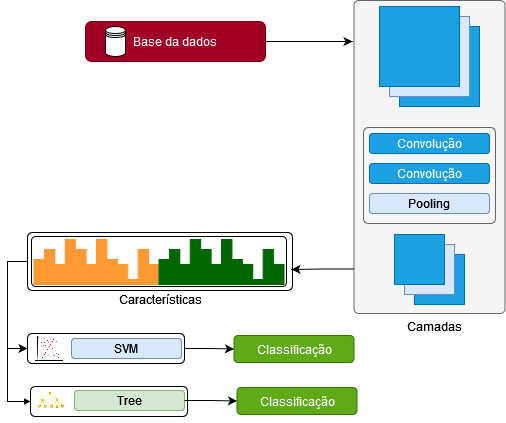
\includegraphics[width=0.5\textwidth]{cnn_extract.png}
\caption{Representação do método proposto nos experimentos}
\label{fig:esquematica_cnn_}
\par\medskip\selectfont\textbf{Fonte:} Elaborada pelo autor (2022) \par\medskip
\end{figure}


\begin{enumerate}
\item Nesta abordagem construímos um modelo de rede neural convolucional tradicional CNN sua arquitetura é mostrada na figura~\ref{fig:arquitetura_cnn_}, foi treinada para classificar as instancias de feijão-fava, encontrando ótimos resultados com mínimo de erro, obtendo valores ótimos de classificação de feijão-fava. % os melhores valores para os filtros no problema de classificação de feijão-fava.
\item Na segunda abordagem o modelo de CNN gerado inicialmente foi utilizado como extrator de características, onde foi removida a camada de classificação softmax. Assim, os valores de ativação dos neurônios da rede que estariam ligados nesta camada são utilizados como entrada à Máquina de Vetores de Suporte (SVM) e tambem para a árvore de decisão como mostra na figura~\ref{fig:esquematica_cnn_}.
% \item Na terceira e última abordagem é utilizado o modelo CNN gerado na primeira abordagem como extrator de características, foi removida a última camada a de classificação softmax. Assim, os valores de ativação dos neurônios da rede que estariam ligados nesta camada são utilizados como entrada em uma árvore de decisão para a classificação como mostra na figura~\ref{fig:Arquitetura-CNN}.
\end{enumerate}



\subsection{SVM}

O SVM tem o objetivo encontrar o hiperplano de separação ideal o qual maximiza a margem da base de treinamento buscando o equilíbrio entre ambos os erros, minimizando o excesso de ajustes (overfitting) e melhorando a capacidade de generalização~\cite{vapnik1995nature}. 

Utilizando o modelo de CNN descrito a cima como extrator de característica, onde foi removendo sua última camada a de classificação softmax. Assim, os valores de ativação dos neurônios da rede que estariam ligados nesta camada são utilizados como entrada em uma Maquina de Vetores de Suporte (SVM) para a classificação. A tabela~\ref{tabela:hiperparametros_svm} mostra as distribuições dos hiperparâmetros que foram utilizado selecionados pela busca aleatória  ~\cite{Bergstra_James}.

\begin{table}[H]
\centering
\caption{Hiperparâmetros}
\label{tabela:hiperparametros_svm}
\def\arraystretch{1.2}
\begin{tabular}{@{}lrrr@{}}
\toprule
{\textbf{Algoritimos}} & {\textbf{Hiperparâmetros}} & {\textbf{Distribuição de Probabilidade}}  \\
\midrule
CNN SVM & C &  uniforme em [0.0001; 100.00] \\ 
CNN SVM & kernel &  uniforme em \{poly, rbf, linear\} \\ 
CNN SVM & Grau do polinômio & uniforme em [2; 5] \\ 
CNN SVM & $\gamma$ & uniforme em [0.0001; 100.00] \\ 
\bottomrule
\end{tabular}
\end{table}

Os Resultados obtidos através da matriz de confusão, que das 413 instâncias acertou 197 da classe fava cearense e 201 de fava orelha de vó e teve 6 erros obtendo uma precisão de 0.98, com uma cobertura de 0.99 e a Área sob a curva AUC de 0.988.

Na tabela~\ref{tabela:hiperparametros_best_models_svm_}, mostra os hiperparâmetros relacionado ao modelo que obteve os melhores resultados, obtidos através da seleção de modelos.

\begin{table}[H]
\centering
\caption{Hiperparâmetros do Melhor Modelo SVM}
\label{tabela:hiperparametros_best_models_svm_}
\def\arraystretch{1.2}
\begin{tabular}{@{}lrrr@{}}
\toprule
{\textbf{Algoritimos}} & {\textbf{Hiperparâmetros}} & {\textbf{Variação}}  \\
\midrule
CNN SVM & C & $2.91x10^{1}$ \\ %29.115026486768507 \\ 
CNN SVM & kernel & poly \\ 
CNN SVM & Grau do polinômio & 2 \\ 
CNN SVM & $\gamma$  & 
 $4.78x10^{-4}$ \\
% 0.0004780004165163952 \\
\bottomrule
\end{tabular}
\end{table}

\subsection{Árvore de decisão}

As árvores são formadas por nós, que armazenam informação (perguntas). O nó raiz é o nó que possui maior nível hierárquico e, a partir dele, ramificam-se os nós filhos. O nó que não possui filhos é conhecido como nó folha ou terminal. Para se gerar um novo galho é necessário que ocorra um separação dos dados no plano. No entanto, essa separação precisa melhorar a separação anterior, caso contrário não faz sentido separar mais os dados.

Da mesma forma, Utilizando CNN com extrator de característica, removendo sua última camada a de classificação softmax. Assim, os valores de ativação dos neurônios da rede que estariam ligados nesta camada são utilizados na entrada de uma Árvore de Decisão para a classificação como mostra na figura~\ref{fig:esquematica_cnn_}. A tabela~\ref{tabela:hiperparametros_tree}  mostra as distribuições dos hiperparâmetros que foram utilizado selecionados pela busca aleatória  ~\cite{Bergstra_James}.

\begin{table}[H]
\centering
\caption{Hiperparâmetros}
\label{tabela:hiperparametros_tree}
\def\arraystretch{1.2}
\begin{tabular}{@{}lrrr@{}}
\toprule
{\textbf{Algoritimos}} & {\textbf{Hiperparâmetros}} & {\textbf{Distribuição de Probabilidade}}  \\
\midrule
CNN TREE & critério &  uniforme em \{gini, entropy\} \\ 
CNN TREE & divisor & uniforme em \{best, random\} \\ 
CNN TREE & amos mín dividida & uniforme em [0; 1] \\ 
CNN TREE & amos mín por folha & uniforme em [0.00000; 0.5] \\ 
CNN TREE & máx de nós por folha & uniforme em [1; 1000] \\ 
CNN TREE & profundidade máx & uniforme em [1; 1000]\\ 
\bottomrule
\end{tabular}
\end{table}

Os Resultados obtidos através da matriz de confusão, que das 413 instâncias acertou 186 da classe fava Cearense e 216 de fava Orelha de Vó e teve 11 erros obtendo uma precisão de 0.96, com uma cobertura de 0.98 e a Área sob a curva AUC de 0.979.

% \begin{figure}[H]
% \centering
% \includegraphics[width=1.0\textwidth]{img/CNN_TREE.png}
% \caption{CNN TREE Resultados }
% \label{fig:tree_result}
% \end{figure}

Na tabela~\ref{tabela:hiperparametros_best_models_tree_}, mostra os hiperparâmetros relacionado ao modelo que obteve os melhores resultados, obtidos através da seleção de modelos.

\begin{table}[H]
\centering
\caption{Hiperparâmetros do Melhor Modelo Arvore}
\label{tabela:hiperparametros_best_models_tree_}
\def\arraystretch{1.2}
\begin{tabular}{@{}lrrr@{}}
\toprule
{\textbf{Algoritimos}} & {\textbf{Hiperparâmetros}} & {\textbf{Variação}}  \\
\midrule
CNN TREE & criterion & gini \\ 
CNN TREE & max depth &   436 \\ 
CNN TREE & max leaf nodes & 861 \\ 
CNN TREE & min samples leaf & $9.17x10^{-2}$ \\ % 0.0917183949330819 \\  
CNN TREE & min samples split & $7.79x10^{-1}$ \\ %  0.7796910002727693 \\ 
CNN TREE & splitter & best \\ 
\bottomrule
\end{tabular}
\end{table}


\subsection{VGGNet}

Este experimento foi realizado de forma adicional, utilizando Transferência de Aprendizado (transfer learning) como arquitetura vgg16 treinados com os pesos da imagenet \cite{ImageNet}, com extrator de característica, da mesma forma como foi feito com o modelo de CNN descrito a cima, removendo a camada totalmente conectada e substituindo por uma arquitetura de MLP, com a mesma configuração utilizada nas camadas totalmente conectadas da CNN. A tabela~\ref{tabela:hiperparametros_vgg} mostra as distribuições dos hiperparâmetros que foram utilizado selecionados pela busca aleatória  ~\cite{Bergstra_James}.

\begin{table}[H]
\centering
\caption{Hiperparâmetros}
\label{tabela:hiperparametros_vgg}
\def\arraystretch{1.2}
\begin{tabular}{@{}lrrr@{}}
\toprule
{\textbf{Algoritimos}} & {\textbf{Hiperparâmetros}} & {\textbf{Distribuição de Probabilidade}}  \\
\midrule
CNN VGG16 & dropout & uniforme em \{0.5, 0.6, 0.7, 0.8, 0.9, 0.10, 0.11, 0.12\} \\ 
CNN VGG16 & neurônios & uniforme em \{32, 64, 128, 256\} \\ 
CNN VGG16 & ativação & uniforme em \{relu, sigmoid\} \\ 
CNN VGG16 & épocas & uniforme em [50; 500] \\ 
CNN VGG16 & tamanho do batch & uniforme em \{16, 32, 64, 128\} \\ 
CNN VGG16 & otimizador & uniforme em \{adam, sgd, rmsprop, nadam\} \\ 
\bottomrule
\end{tabular}
\end{table}

Os Resultados obtido com está abordagem, através da matriz de confusão, que das 413 instâncias acertou 186 da classe fava cearense e 212 de fava Orelha de Vó e teve 15 erros obtendo uma precisão de 0.95, com uma cobertura de 0.96 e a Área sob a curva AUC de 0.974.

Na tabela~\ref{tabela:hiperparametros_best_models_vgg_}, mostra os hiperparâmetros relacionado ao modelo que obteve os melhores resultados, obtidos através da seleção de modelos.

\begin{table}[H]
\centering
\caption{Hiperparâmetros do Melhor Modelo VGG16}
\label{tabela:hiperparametros_best_models_vgg_}
\def\arraystretch{1.2}
\begin{tabular}{@{}lrrr@{}}
\toprule
{\textbf{Algoritimos}} & {\textbf{Hiperparâmetros}} & {\textbf{Variação}}  \\
\midrule
VGG16 MLP & épocas & 166 \\ 
VGG16 MLP & tamanho do batch & 32\\ 
VGG16 MLP & otimizador & nadam \\
VGG16 MLP & ativação & relu \\
VGG16 MLP & neurônios & 64 \\
VGG16 MLP & dropout & 0.1 \\
\bottomrule
\end{tabular}
\end{table}






















% \section{Seleção de Modelos}

% Para o ambiente experimental utilizada para o desenvolvimento a linguagem Python. Para realizar a implementação dos experimentos e executar os algoritmos de Aprendizado de Máquina foram utilizadas as bibliotecas Scikit-Learn~\footnote{ \url{https://scikit-learn.org/}}, Keras~\footnote{ \url{https://keras.io/}} e Tensor Flow~\footnote{ \url{https://tensorflow.org/}}. No inicio, os experimentos foram executados no Colab em sua versão gratuita, em que é disponibilizado 12GB de memória RAM e GPU no modelo K80. Mais, suas limitações impediam a execução, sendo necessário utilizar o Google Colab~\footnote{ \url{https://colab.research.google.com/}}, na sua versão Pro, o qual é fornecido 25GB de memória RAM, com GPU T4 ou P100.

% Para otimizar a seleção dos modelos utilizou-se a busca aleatória \textit{RandomSearchCV} para a escolha do melhor conjunto de hiperparâmetro, esse método possui um grande benefício significativo. De acordo com \cite{Bergstra_James}, os parâmetros escolhidos utilizando a técnica de busca em grade aleatória é mais eficaz que as demais técnicas, pois não tenta todas as combinações hiperparâmetros. Ela é capaz de encontrar modelos tão bons ou melhores em uma pequena fração do tempo de computação. Esta é uma vantagem muito significativa devido às limitações dos recursos de hardware disponíveis para o experimento. Utiliza uma combinação de hiperparâmetros aleatória para treinar cada modelo, com o mesmo número de \textbf{k-folds} em \textit{k}=5 para todas as abordagens,  e utilizou \textit{n}=50 esse n é o numero de combinações utilizadas na busca aleatória. 

% A tabela~\ref{tabela:hiperparametros} mostra as distribuições dos hiperparâmetros que foram utilizados na busca aleatório.

% \begin{table}[H]
% \centering
% \caption{Hiperparâmetros}
% \label{tabela:hiperparametros}
% \def\arraystretch{1.2}
% \begin{tabular}{@{}lrrr@{}}
% \toprule
% {\textbf{Algoritimos}} & {\textbf{Hiperparâmetros}} & {\textbf{Distribuição de Probabilidade}}  \\
% \midrule
% % CNN MLP & dropout & uniforme em \{0.5, 0.6, 0.7, 0.8, 0.9, 0.10, 0.11, 0.12\} \\ 
% % CNN MLP & neurônios & uniforme em \{32, 64, 128, 256\} \\ 
% % CNN MLP & ativação & uniforme em \{relu, sigmoid\} \\ 
% % CNN MLP & épocas &  uniforme em [50; 500] \\ 
% % CNN MLP & tamanho do batch &  uniforme em \{16, 32, 64, 128\} \\ 
% % CNN MLP & otimizador &  uniforme em \{adam, sgd, rmsprop, nadam\} \\ 
% % \hline 

% CNN SVM & C &  uniforme em [0.0001; 100.00] \\ 
% CNN SVM & kernel &  uniforme em \{poly, rbf, linear\} \\ 
% CNN SVM & Grau do polinômio & uniforme em [2; 5] \\ 
% CNN SVM & $\gamma$ & uniforme em [0.0001; 100.00] \\ 
% \hline CNN TREE & critério &  uniforme em \{gini, entropy\} \\ 
% CNN TREE & divisor & uniforme em \{best, random\} \\ 
% CNN TREE & amos mín dividida & uniforme em [0; 1] \\ 
% CNN TREE & amos mín por folha & uniforme em [0.00000; 0.5] \\ 
% CNN TREE & máx de nós por folha & uniforme em [1; 1000] \\ 
% CNN TREE & profundidade máx & uniforme em [1; 1000]\\ 
% \hline CNN VGG16 & dropout & uniforme em \{0.5, 0.6, 0.7, 0.8, 0.9, 0.10, 0.11, 0.12\} \\ 
% CNN VGG16 & neurônios & uniforme em \{32, 64, 128, 256\} \\ 
% CNN VGG16 & ativação & uniforme em \{relu, sigmoid\} \\ 
% CNN VGG16 & épocas & uniforme em [50; 500] \\ 
% CNN VGG16 & tamanho do batch & uniforme em \{16, 32, 64, 128\} \\ 
% CNN VGG16 & otimizador & uniforme em \{adam, sgd, rmsprop, nadam\} \\ 
% \bottomrule
% \end{tabular}
% \end{table}

% O modelo de rede neural convolucional utilizado como base na comparação com outros métodos tem a seguinte arquitetura mostrada na figura~\ref{fig:arquitetura_cnn}, e este mesmo modelo foi utilizado como extrator de características para os classificadores SVM e Árvore de decisão, após ter sido removida a camada de classificação softmax.

% \begin{figure}[H]
% \centering
% 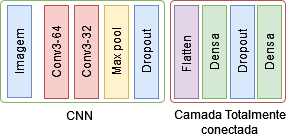
\includegraphics[width=0.5\textwidth]{CNN.png}
% \caption{Arquitetura da CNN}
% \label{fig:arquitetura_cnn}
% \par\medskip\selectfont\textbf{Fonte:} Elaborada pelo autor (2022) \par\medskip
% \end{figure}

% A extração das características usando a CNN pré treinada consiste inicialmente em carregar uma arquitetura de um modelo rede neural convolucional já treinada com o conjunto de imagens de feijão-lima, aproveitar o treinamento básico de suas características. Depois é removido seu classificador, para a saída da rede ser um vetor de características.

% Como mostra a figura~\ref{fig:esquematica_cnn}, todo o fluxo dos dados que inicia na camada de convolução passa na camada de pooling onde é extraído os mapas de características que por sua vez passa por uma camada de flatter onde foi transformado em vetor de características é utilizado como entrada nos modelos de Maquina de Vetores de Suporte (SVM) e Árvore de Decisão.

% \begin{figure}[H]
% \centering
% 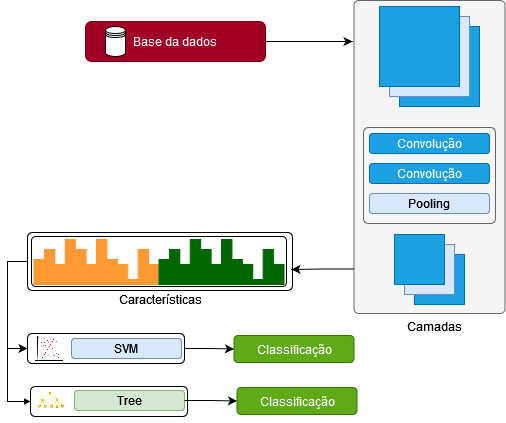
\includegraphics[width=0.5\textwidth]{cnn_extract.png}
% \caption{Representação do método proposto nos experimentos}
% \label{fig:esquematica_cnn}
% \par\medskip\selectfont\textbf{Fonte:} Elaborada pelo autor (2022) \par\medskip
% \end{figure}

\label{sec:metodologia}

\section{Conclusão}

Foi possível perceber que todos os métodos testados erraram poucas instância, indicando uma boa precisão nas classificações no experimento como mostra na tabela~\ref{tabela:metricas}. De modo geral, os resultados com SVM foram superiores aos com o classificador baseado em Softmax e Árvore de decisão. Onde a máquina de vetores de suporte (SVM) obteve uma precisão de 0.98 com 6 erros apenas 6 instâncias foi onde se obteve os melhores resultados seguido pela Árvore de decisão que apresentou uma precisão de 0.96.

\begin{table}[H]
\centering
\caption{Contem as métricas precisão e Sensibilidade}
\label{tabela:metricas}
\def\arraystretch{1.2}
\begin{tabular}{@{}lrrrrrrr@{}}
\toprule
{\textbf{Algoritimos}} & {\textbf{Precisão}} & {\textbf{Cobertura }} & {\textbf{AUC-ROC}}\\
\midrule
CNN & 0.946429 & 0.968037 & 0.966  \\ 
CNN SVM & 0.981308 & 0.990566 & 0.988  \\ 
CNN TREE & 0.964286 & 0.986301 & 0.979 \\
VGG16 MLP & 0.958762 & 0.963730 & 0.974 \\
% VGG16 & 0.963636 & 0.968037 \\ 
\bottomrule
\end{tabular}
\end{table}

Os sistemas de visão computacional têm sido cada vez mais utilizados na agricultura facilitando a tomada de decisão dos agricultores. O presente trabalho apresentou um método para identificação de espécies e classificação de mudas de feijão-fava. Neste trabalho, quatro modelos foram comparados com a finalidade de determinar qual seria o melhor classificador. Como visto no capítulo anterior, a junção de SVM com as camadas de convolução na etapa de extração de características se mostrou eficaz, com apenas 6 erros obtendo uma precisão de 0.98 e cobertura de 0.99.

Como trabalhos futuros, pretendemos explorar mais variedades como boca-de-moça, branquinha, mororó, olho-de-ovelha, olho-de-peixe, raio-de-sol, rajada vermelha, rajada preta. Obter recursos de hardware mais robustos, para estender a seleção de modelos.

\label{sec:conclusao}
% ---------------------------------
\bibliographystyle{unsrt}
\bibliography{sbc-template}
\end{document}